\documentclass[11pt]{article}
\usepackage{amsmath}
\usepackage{amssymb}
\usepackage{graphicx}
\usepackage{epstopdf}
\usepackage{inputenc}
\usepackage{float}
\usepackage{geometry}
\graphicspath{ {../results/plots} }
\usepackage{csvsimple}
\usepackage{hyperref}
\usepackage{listings}
\usepackage{cleveref}
\usepackage{lscape}

\newcommand{\betaEst}{0.184}
\newcommand{\rhoEst}{364}
\newcommand{\repEst}{6.04}
\newcommand{\RN}[1]{%
  \textup{\uppercase\expandafter{\romannumeral#1}}%
}

\title{SARS-CoV-2 Outbreak Reduction: Executive Summary}

\author{
        Forrest Koch \\
        forrest.koch@unsw.edu.au \\
        University of New South Wales \\
}
\date{\today}

\begin{document}
\maketitle

\begin{abstract}
\end{abstract}

\section{Executive Summary}
blah
\section{Project Scope}
blah
\section{Results}

\section{Recommendations}

\section{Limitations}

\section{Future Work}
    %\begin{figure}
    %    \centering
    %    \includegraphics[scale=0.75]{flow_diagram}
    %    \caption{Flow Diagram of Hepatitis E compartmental model. *$H_{\RN{2}}$ is the Holling functional of the second kind.}
    %    \label{flow_diagram}
    %\end{figure}

    %\begin{table}
    %    \begin{tabular}{ c c l l}
    %        Parameter & Value & Description & Determination\\
    %        \hline \\
    %        $\alpha$    & 0.125     & Proportion of symptomatic/clinical cases       & Assumed \\
    %        $\beta$     & \betaEst  & Rate of transmission from infectious          & MLE* \\
    %    \end{tabular}
    %    \caption{Table of model parameters. All rates are given in weeks (i.e the infectious period is $\frac{1}{\gamma} = 5$ weeks). *Maximum Likelihood Estimation} 
    %    \label{parameter_table}
    %\end{table}
        %\subsubsection{Parameter Definition}
\section{Acknowledgements}

\bibliographystyle{unsrt}
\bibliography{main}

\section{Technical Appendix}

\subsection{Model Summary}
\lstinputlisting[basicstyle=\tiny]{../results/stansummary-clean.txt}

\subsection{Calculation of $R_0$}
The closed form for this model is complicated to write down, so the following
code was used for calculations. With $\beta=0.1154$, we get $R_0\approx1.29$.

\lstinputlisting[language=python,basicstyle=\tiny]{../src/basic_reproduction_number.py}


\subsection{Supplemental Figures}
    \begin{figure}
        \centering
        \includegraphics[scale=0.75]{flow_diagram}
        \caption{Flow diagram of the SLAPIR compartmental model. Multiple compartments are leveraged to enforce a gamma 
        distribution on total time spent in the compartment.  Infected individuals go through a latent period (L1-4) followed by
        either an asymptomatic period (A1-12, probability = 20\%) a pre-symptomatic/symptomatic period (P1-2/I1-10, probability = 80\%).}
        \label{flow_diagram}
    \end{figure}
    \begin{figure}
        \centering
        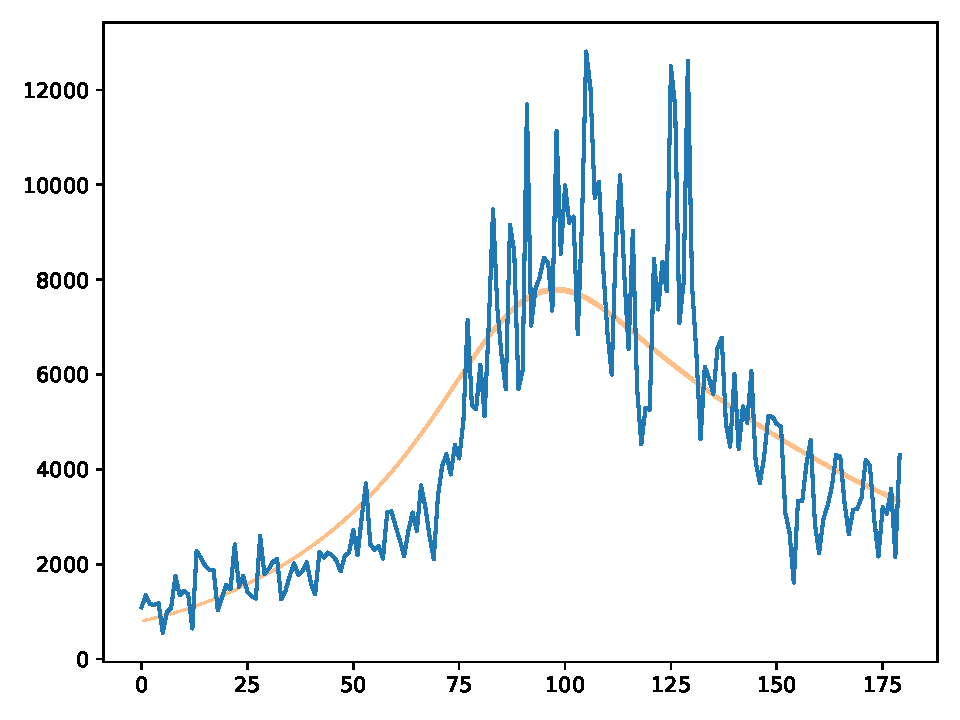
\includegraphics[scale=0.75]{model_fit}
        \caption{Plot of daily reports of Covid cases in California over 180 days starting from 07/04/20-04/10/20 (orange) 
        and the incidence predicted by the model fit (blue).}
        \label{model_fit}
    \end{figure}
    \begin{figure}
        \centering
        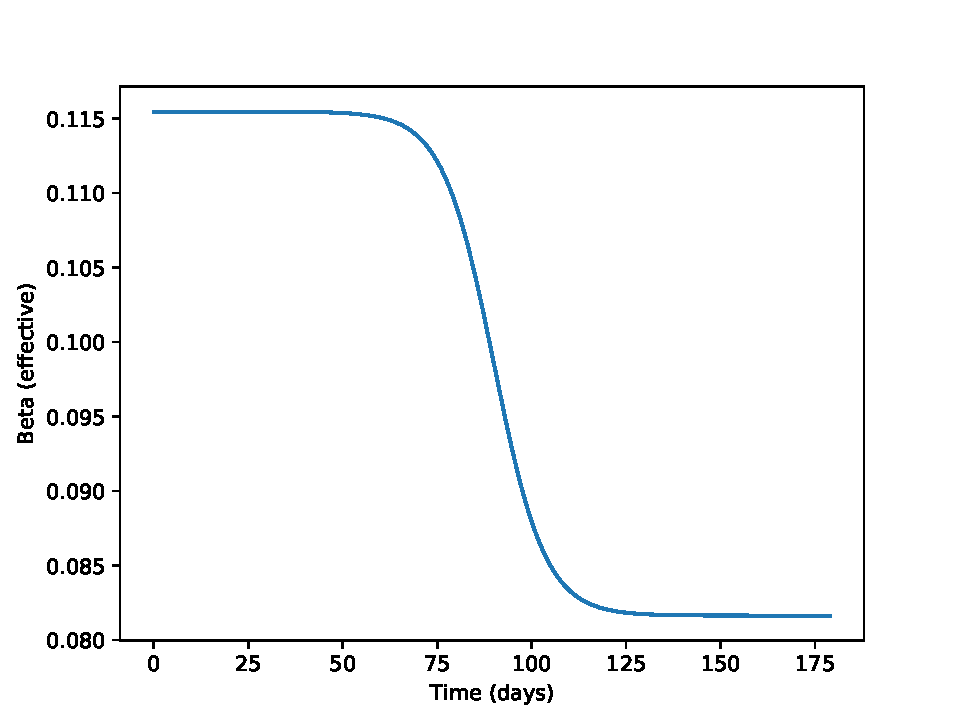
\includegraphics[scale=0.75]{beta_over_time}
        \caption{Plot of the estimated change it $\beta_{eff}$ over the period studied.}
        \label{beta_over_time}
    \end{figure}
    \begin{figure}
        \centering
        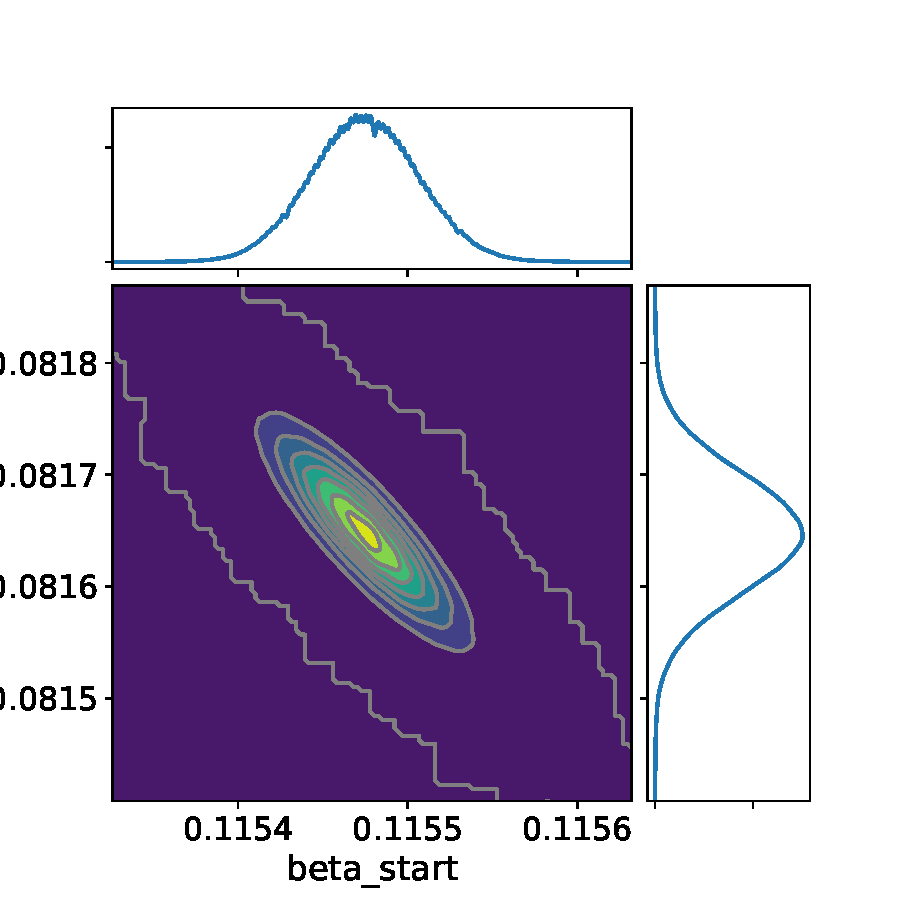
\includegraphics[scale=0.75]{model_joint_betas}
        \caption{Plot of the joint density of $\beta_{start},\beta_{end}$ output by the model.}
        \label{model_joint_betas}
    \end{figure}
    \begin{landscape}
    \begin{figure}
        \centering
        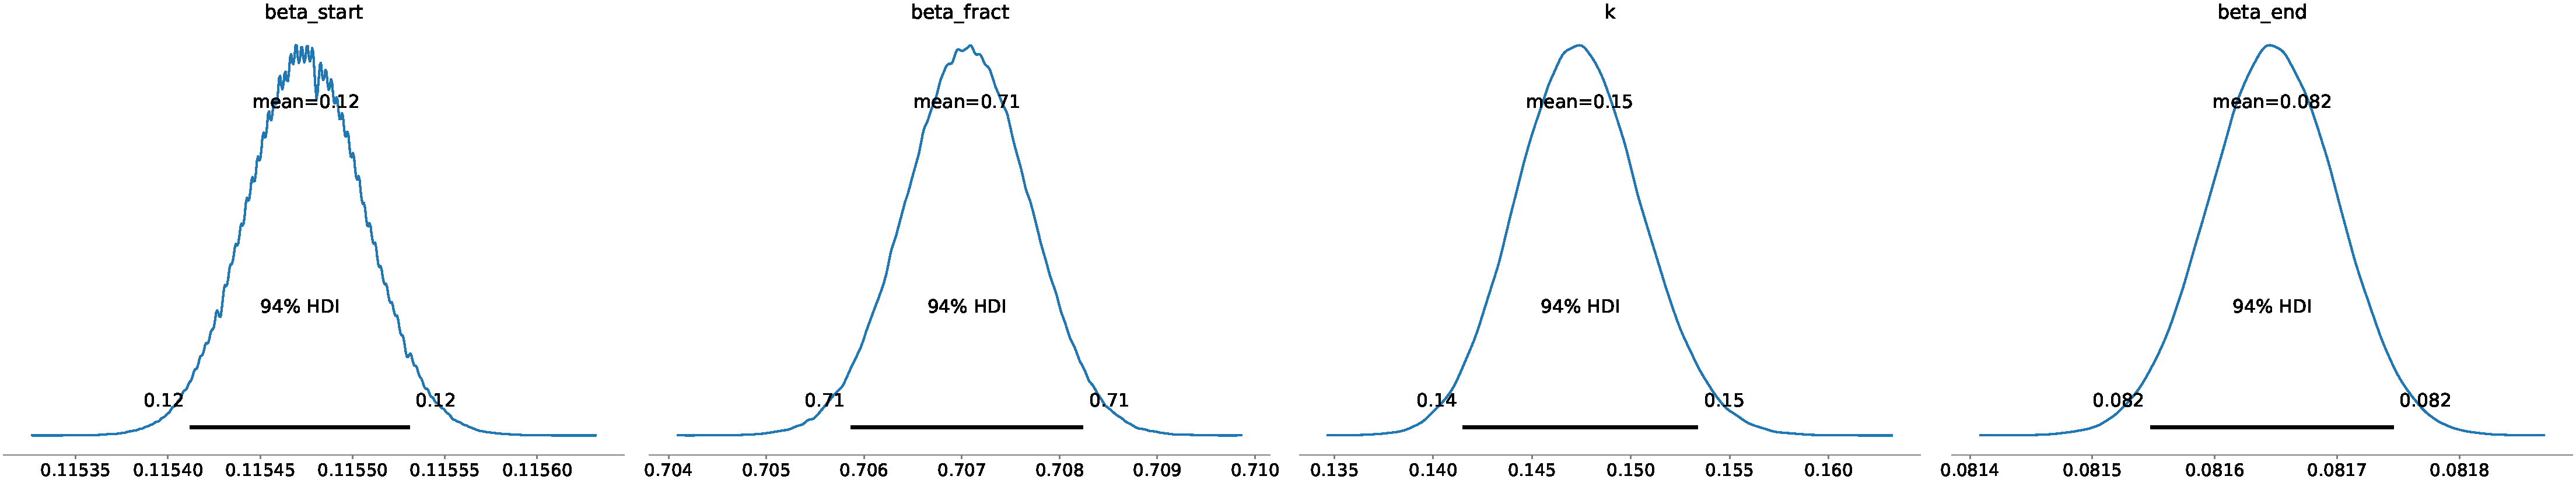
\includegraphics[scale=0.2]{model_posterior}
        \caption{Posterior density plots showing the HDI interval for each estimated parameter.}
        \label{model_posterior}
    \end{figure}
    \begin{figure}
        \centering
        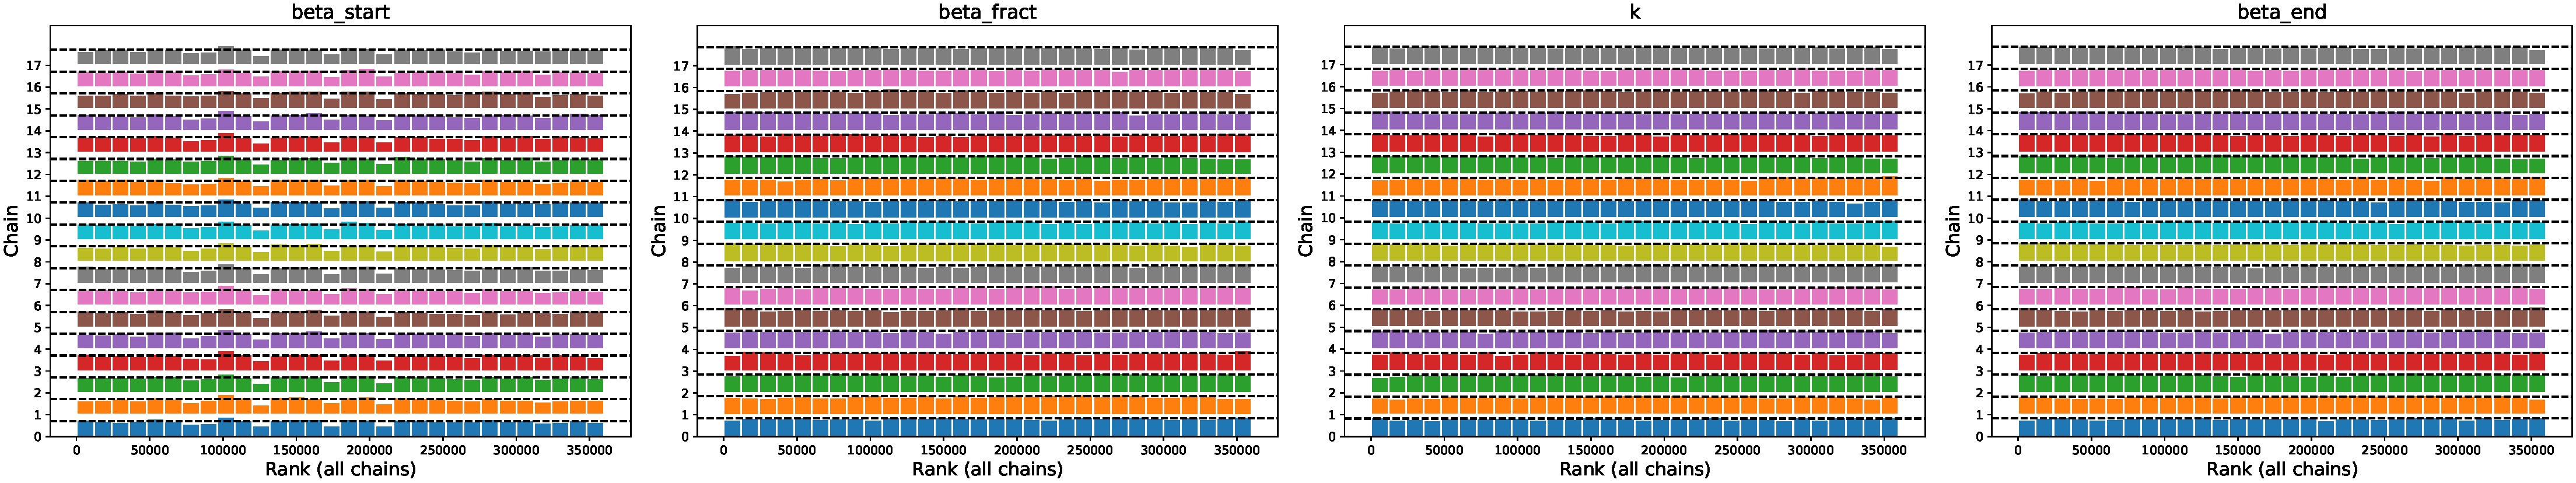
\includegraphics[scale=0.2]{model_rank}
        \caption{Diagnostic plots showing parameter rank for each chain.}
        \label{model_rank}
    \end{figure}
    \begin{figure}
        \centering
        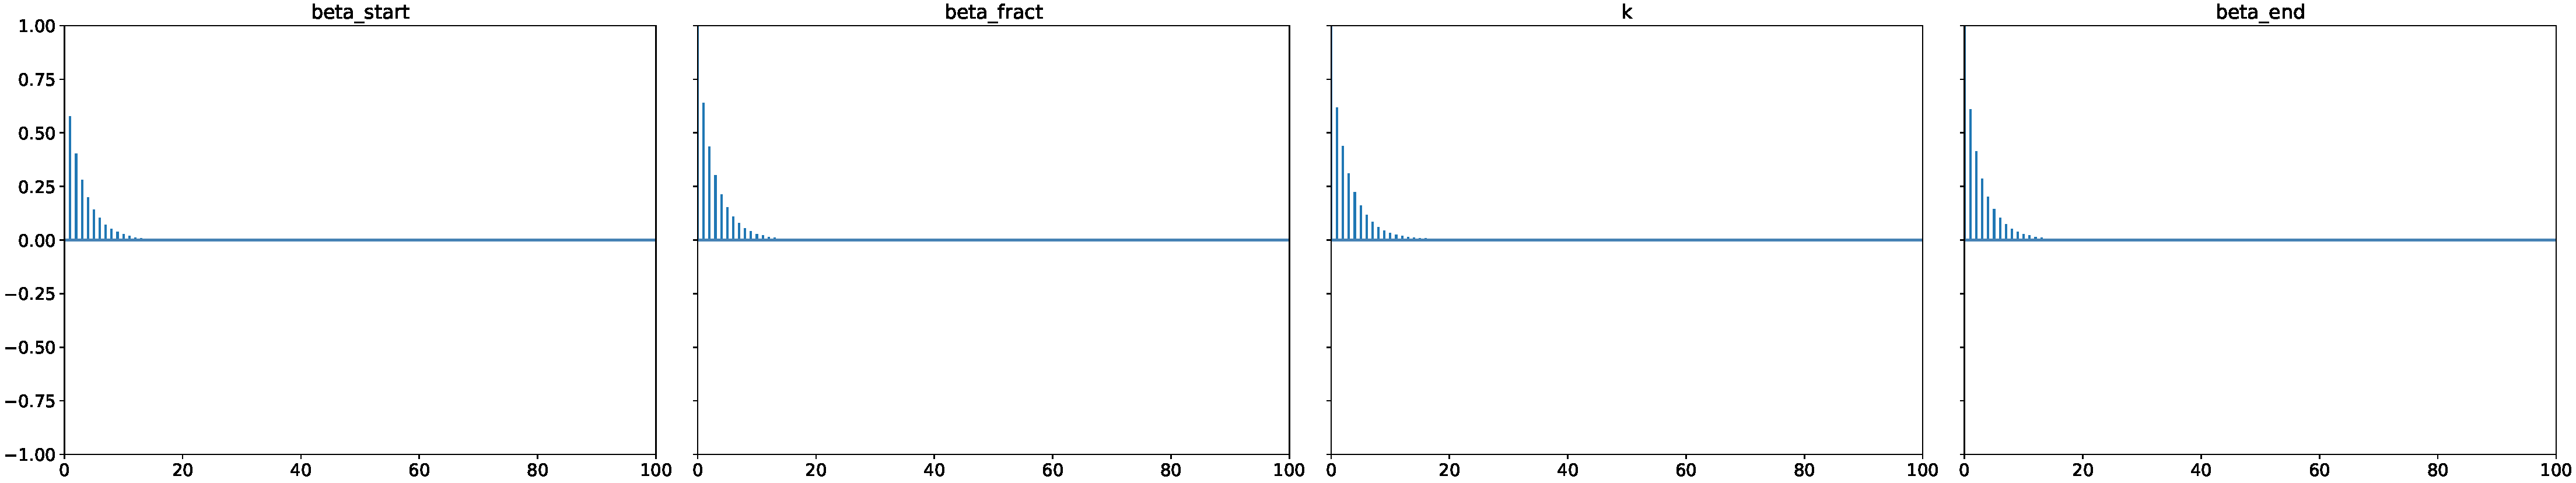
\includegraphics[scale=0.2]{model_autocorrelation}
        \caption{Diagnostic plot showing autocorrelation across all chains.}
        \label{model_autocorrelation}
    \end{figure}
    \end{landscape}

\end{document}
